\chapter{Context Free Grammars}
	\section{Preliminar definitions}
		Regular expressions as a tool to generate languages are not enough powerful. 
		Super simple languages like "all words followed by their reverse" or "concatenation of two strings of the same length" cannot be generated.

		Context Free grammars are defined by means of four entities
		\begin{itemize}
			\item $V$: \emph{non-terminal alphabet}, is a set of \emph{non-terminal symbols (or syntactic classes)}
			\item $\sum$: \emph{terminal alphabet}, is the set of the \emph{characteres} that costitute the phrases
			\item $P$: is a set of \emph{syntactic rules} (also called \emph{production rules} or simply \emph{rules})
			\item $S \in V$ is a particular non-terminal, called axiom
		\end{itemize}
		One particular nonterminal is choosen as starter (or axiom).
		A Rule is an ordered pair with a left side and a right side: left side can contain only nonterminals, right side both terminals and nonterminals. 
		
		In order to define a language, one can use RULES that, after repeated application, allow to generate all and only the phrases of the language
		The set of such rules constitutes a GENERATIVE GRAMMAR (or SYNTAX).

		\begin{definition}[Regular Language]
			A set of rules generating all the possible strings belong to the language.
		\end{definition}


		\subsection{Rule Classification}
			Lowercase or greek letters: terminals.\\
			Uppercase letters: terminals.
			\begin{definition}[Recursive]
				A $\rightarrow$ $\alpha$ A $\beta$ 
			\end{definition}
			\begin{definition}[Left recursive]
				A $\rightarrow$ A $\beta$ 
			\end{definition}
			\begin{definition}[Right recursive]
				A $\rightarrow$ $\alpha$ A
			\end{definition}
			\begin{definition}[Copy]
				A $\rightarrow$ B
			\end{definition}
			\begin{definition}[Linear]
				At most one nonterminal on the right side.
			\end{definition}
			\begin{definition}[Right Linear]
				Linear + nonterminal is suffix.
			\end{definition}
			\begin{definition}[Left Linear]
				Linear + nonterminal is prefix.
			\end{definition}
			\begin{definition}[Chomsky]
				Right side is either two nonterminals or a terminal.
			\end{definition}
			\begin{definition}[Greibach normal]
				Right side starts with a terminal symbol.
			\end{definition}
			\begin{definition}[Operator normal]
				A $\rightarrow$ B c D.
			\end{definition}
    \section{Grammar Cleaning}
        Writing a grammar following non-grammar rules (so doing it for a purpose and not for its own sake) can lead to useless rules or unreachable 
		terminals or nonterminals. This is prevented by the Grammar Cleaning algorithm:
            \begin{enumerate}
                \item Compute the well-defined nonterminals (the ones that are "reachable from the production")
                \item From the well defined nonterminals build the production tree (such a rare technique in computer science) and check if there are nonterminals in 
				the nonterminal alphabet that are not reachable from the axiom.
                \item (Optional but useful) Check for circular derivation like A $\rightarrow$ A $\rightarrow$ x
            \end{enumerate}
    
    \section{Infinite Grammars}
        A grammar is said to be infinite\\
        $\Leftrightarrow$\\
        A grammar has a recursive production\\\\
        The grammar is assumed to be clean and free from circular derivation. 
       
    \section{Syntax Trees}
    	The production procedure can be visualized by a tree (how strange) where every arch represents a symbol of the right part (or a choice for it). They're 
		regular trees (so connected directed acyclic graphs) but the nodes on the same level (or at least sons of the same father) are ordered from left to right.

    	The degree or arity of a node is the number of its \emph{siblings} (and not of his sons, that's more intuitive). The \emph{frontier} of the tree is the 
		sequence of all leaves. \underline{A syntax tree has the axiom as the root and a sentence as the frontier}.

    	\textbf{Remember:} a syntax tree represents \textbf{a single production} and not all possible ones.
	
	\section{Ambiguity}\label{sec:ambig}
		Ambiguity\index{Ambiguity} in grammars is similar to the ambiguity for regular expressions. The definition is pretty much the same: a sentence is ambiguous 
		if it admits several different syntax trees.

		Syntactic ambiguity (the only of interest when studying formal languages) is the kind of ambiguity that derives from the \emph{structure} of the production, 
		rather than the effective meaning it carry.% //TODO metti in risalto sta cosa

		The formal problem of discovering/computing the ambiguity of a grammar is an undecidable one. This is in practice not a great problem: heuristics to check 
		if a given grammar is ambiguous exists, but most importantly the grammar designer should keep in mind (and design accordingly) the said grammar in an 
		unambiguous way.
		
		\subsection{Ambiguous Forms and Remedies}
		% //TODO metti una description o fai capire che stai per elencare i tipi 
			\subsubsection{Bilateral Recursion}
				A bilateral recursion (so a both left and right recursive rule) often leads to ambiguity because there's usually no fixed order of generation 
				of nonterminals.

				This can be usually avoided by splitting the two side recursive rule into more rules each one either right or left recursive.

			\subsubsection{Ambiguity from Union}
				Pretty straightforward: if two different languages can generate the same sentence, the union of these languages is ambiguous by construction.

				To cope with such problem, often a full redesign of the grammars is needed.
			\subsubsection{Ambiguity from Concatenation}
				Concatenating two (or more) languages can be a problem if a suffix of a language is a prefix in a language that follows it.

				To remove this kind of ambiguity, it's sufficent to add an extra separator character between languages.
			\subsubsection{Ambiguity in Conditional Phrase}
				The infamous "dangling else problem" is an ambiguity problem that falls in this category. Generally this kind of ambiguity arises when more 
				variants are accepted for the same language structure, and no particular delimiter for parts is provided.

				Usually removed by adding delimiters (endif, fi)
			\subsubsection{Inherent Ambiguity}
				An inherent ambiguous language is generated by a set of grammar in which \emph{all} the grammars are ambiguous
	
	\section{Closure Property}
		The CF languages (so all languages generated by Context Free grammars) are closed under the operations of
		\begin{itemize}
			\item union
			\item concatenation
			\item star
		\end{itemize}
		
		\subsubsection{Complement and Intersection}
			Let L and L2 be regular languages. Their intersection and the complement of each is still a regular language. (The formal proof utilizes the 
			recognizers automata to prove this).
	
	\section{Equivalence}
	%//TODO metti una fottuta spiegazione su che cose un condensed tree
		Two grammar are said to be equivalent if they define the same language. Two grammars are \emph{strongly} equivalent if they define the same language 
		\textbf{and} they have the same \emph{condensed} \emph{skeleton} \emph{trees}; this means that every production from both grammar is generated 
		"with the same choices".

		Strong equivalence $\Rightarrow$ weak equivalence

		Strong equivalence can be formally proved, while checking for weak equivalence is an undecidable problem.

		\subsubsection{Structural Adequacy}
			The difference between strong and weak equivalence is not only a formal one: if we consider (for example) the generation of arithmetic expression 
			(that should take into account also the operator precedences) only the grammar with the syntax tree that respects the precedences, and all the 
			\emph{strongly equivalent} ones, will be structurally adequate.

				\begin{figure}
					\centering
					\begin{minipage}{0.45\textwidth}
						\centering
						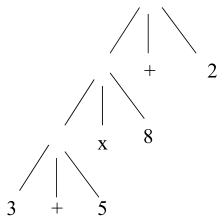
\includegraphics[width=0.9\textwidth]{./images/structAdeq1.png}
				    	\caption{Structurally inadequate syntax tree: it can be seen how the operator precedence is not respected}
					\end{minipage}\hfill
					\begin{minipage}{0.45\textwidth}
						\centering
						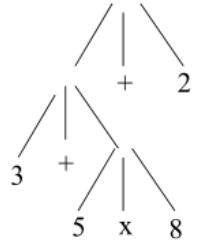
\includegraphics[width=0.9\textwidth]{./images/structAdeq2.png} 
				    	\caption{Structurally adequate tree}
					\end{minipage}
				\end{figure}
			
	\section{Grammar Transformation and Normal Forms}
	%//TODO controllare se c'è tutto, sembra un po' sintetico
		Normal forms are standardized rules. They don't reduce grammar expressiveness of the grammar, and using them does not affect the language iself. They just 
		guide the design process to obtain a grammar with certain properties.

		\subsubsection{Elimination of the axiom from right part}
			Straightforward. Use an additional rule from the axiom to a sub-axiom that is replaced in all other rules.
		\subsubsection{Nullable nonterminals and empty rules}
			A nonterminal is nullable if exists a derivation from said nonterminal to the empty string. To eliminate them, eliminate all the empty productions 
			from the right part of the rules, substituting them with the non-empty sub productions.
		\subsubsection{Copy rules}
			Copy rules are rules in the A $\rightarrow$ B form, with both A and B nonterminals. An algorithm to eliminate copy rules functions this way:
			\begin{enumerate}
				\item A set \emph{Copy(A)} is defined, that contains all the transitive copies of A and A itself
				\item \emph{Copy(A)} is filled with all the nonterminals that are copies (direct or indirect) of A, so that a straight derivation A $\rightarrow$ C 
				exists
				\item The ne set of rules is defined, eliminating all the productions from A to the nonterminals that are in \emph{Copy(A)}.  
			\end{enumerate}
			The above algorithm should take into consideration that a production A $\rightarrow$ BC can be a copy production if either B or C are nullable. Often 
			it's assumed a nonnullable grammar.
		\subsubsection{Recursion conversion}
			Another important class of grammars is the nonleft-recursive. Right recursive grammars are preferred because their laguage is simpler to parse. To 
			transform a left recursive rule to a right ecursive an algorithm has been designed:
			\begin{enumerate}
				\item Identify all the recursive rules of form A $\rightarrow$ A $\gamma$
				\item Add an auxiliary nonterminal X and add the set of rules X $\rightarrow$ $\gamma$ X; the expansion of A becomes A $\rightarrow$ $\alpha$ X, 
				where $\alpha$ is a possible production obtained from A.
			\end{enumerate}
			Now all the immediate l-recursive rules are taken care of.
		\subsubsection{Chomsky normal form}
			Only two possible types of rules: homogeneous binary (nonterminal to two nonterminals) or terminal with singleton right part (nonterminal to single 
			terminal). If the empty string is in the language, it can only appear as an axiomatic production, and the axiom cannot appear in \emph{any} right part.

			Obtaining a Chomsky grammar:
			\begin{enumerate}
				\item all non binary rules are converted to binary: the first non terminal is singled out 
				\item and all the others are replaced by another additional nonterminal, which is added to the nonterminals alphabet and has as production only 
				the one that generates all the leftover nonterminals from passage 1
				\item passages 1 and 2 ainherently recursive
				\item to cope with the rules that have both terminal and non terminals in the right part, the terminals are simple replaced with singleton 
				nonterminals
			\end{enumerate}
		\subsubsection{Greibach and real-time forms}
			Real time grammars are grammars where each right part begins with a terminal symbol. If the additional costraint "the right part could contain exactly 
			one terminal followed by zero or more nonterminals" we obtain a Greibach normal grammar.
			 
	\section{Extended Context Free Grammars}
		They're simply context free grammars (also called Backus Normal Form -> BNF) extended with the regular expression's operation such as star, and union 
		operation. The closure of the CF family under this two operations renders this exension as a merely aesthetic improvement, because the expressiveness 
		remain unchanged.

		The language of a ECF grammar is generated as the one of a CF grammar; the only effect the regular expansion has on the syntactic trees is an augmentation 
		of the breadth and a decrease in the height. This is a further improvement to readability.
	
	\section{Grammar of regular languages}
		As previously stated, regular languages (generated by regular expressions) are a proper subset of context free languages (generated by a context free 
		grammar). This means that there's a one-to-one correlation between regular expression and a grammar that expresses the same language. 
		\subsection{Unilinear Grammars}
		\label{sec:uni_linear_grammars}
			A grammar is said to be linear if every rule of that grammar is in the A $\rightarrow$ uBv form, where A and B non terminals (B can also be $\epsilon$) 
			and u and v terminal symbols.

			If only one of the two terminals is present the grammar is said to be right- or left-linear, wheter the nonterminal is right or left side of the 
			terminal symbol.

			A grammar where all rules are either right or left linear is said unilinear. A strict unilinear grammar has only one terminal per side of the rule.
			\begin{property}[Relation with regular expressions]
				Regular languages are a subset of unilinear languages: REG $\supseteq$ UNI; moreover, from an uniliear grammar we can always derive a regular 
				expression with the same expressiveness $\Rightarrow$ UNI $\supseteq$ REG. We obtain (IMPORTANT) UNI $\equiv$ REG.
			\end{property}
		\subsection{Linear Language equations}\label{sect:linlangeq}
			We want to go from a set of gramamr rules to the complete language generated. To do this we analyse the problem as a problem of languages where the 
			admitted operation is the union of sub-languages.
			Let $n = \lvert V \rvert$ be the number of nonterminals of grammar $G$. Each nonterminal $A_i$ is defined by a set of alternatives:

			$$Ai \longrightarrow a A_1 \vert b A_1 \vert \cdots \vert a A_n \vert b A_n \vert \cdots \vert A_1 \vert \cdots \vert A_n \vert \varepsilon$$
			some of which may also be missing. We write the corresponding linear equation:
			$$L_{A_i} = a L_{A_1} \bigcup b L_{A_1} \bigcup \cdots \bigcup a L_{A_n} \bigcup b L_{A_n} \bigcup \cdots\bigcup L_{A_1} \bigcup \cdots \bigcup 
			L_{A_n} \bigcup \varepsilon$$
			The last term disappears if the rule does not contain the alternative $A_i \rightarrow\varepsilon$.
			
			Practical example: \ref{ese:linlangeq}.